\chapter{Umsätze importieren} \label{chap:import}

Über die Ansicht "`Umsätze importieren"' können Kontoauszüge im CSV-Format importiert werden. Aktuell werden ausschließlich Dateien im Exportformat der ING verarbeitet. Die Ansicht ist im Menü unter "`Daten $\rightarrow$ Importieren"' zu finden.

\section{Ablauf: Umsätze importieren}

Eine CSV-Datei kann über den Button "`Datei auswählen"' oder per Drag \& Drop (in jeder Ansicht) importiert werden. Dann werden die gefundenen Umsätze in einer Tabelle angezeigt (s. Abbildung \ref{fig:ImportView}). Sobald eine Importdatei geöffnet wird, findet eine Zuordnung der gefunden Umsätze zu den \textit{wiederkehrenden Umsätzen} im System statt. Umsätze, die bereits importiert wurden, werden standardmäßig nicht importiert und mit einer entsprechenden Anmerkung versehen.

Sollte ein Umsatz nicht automatisch einem wiederkehrenden Umsatz zugeordnet werden -- da die Importregeln nicht greifen oder keine konfiguriert wurden --, kann eine manuelle Zuordnung über die Zellen der Spalte "`Wiederkehrende Umsätze"' vorgenommen werden. Per Doppelklick auf die Zelle öffnet sich ein Dropdown-Menü mit allen wiederkehrenden Umsätzen im System.

Sollte im System kein passender wiederkehrender Umsatz zu einem realen Umsatz im Import existieren, so kann ein passender aus der Ansicht "`Umsätze importieren"' heraus angelegt werden, indem ein Rechtsklick auf der entsprechenden Zeile der Tabelle ausgeführt wird. 

Sollten die Zuordnungen soweit korrekt sein, können die ausgewählten Umsätze mittels Klick auf den Button "`Ausgewählte importieren"' importiert werden. Dann wird für jeden realen Umsatz ein (einzigartiger) Umsatz im System angelegt, der ggf. mit einem wiederkehrenden Umsatz verknüpft ist, sofern er einem mittels der Importregeln zugeordnet werden konnte.


\begin{figure}[ht!]
	\centering
	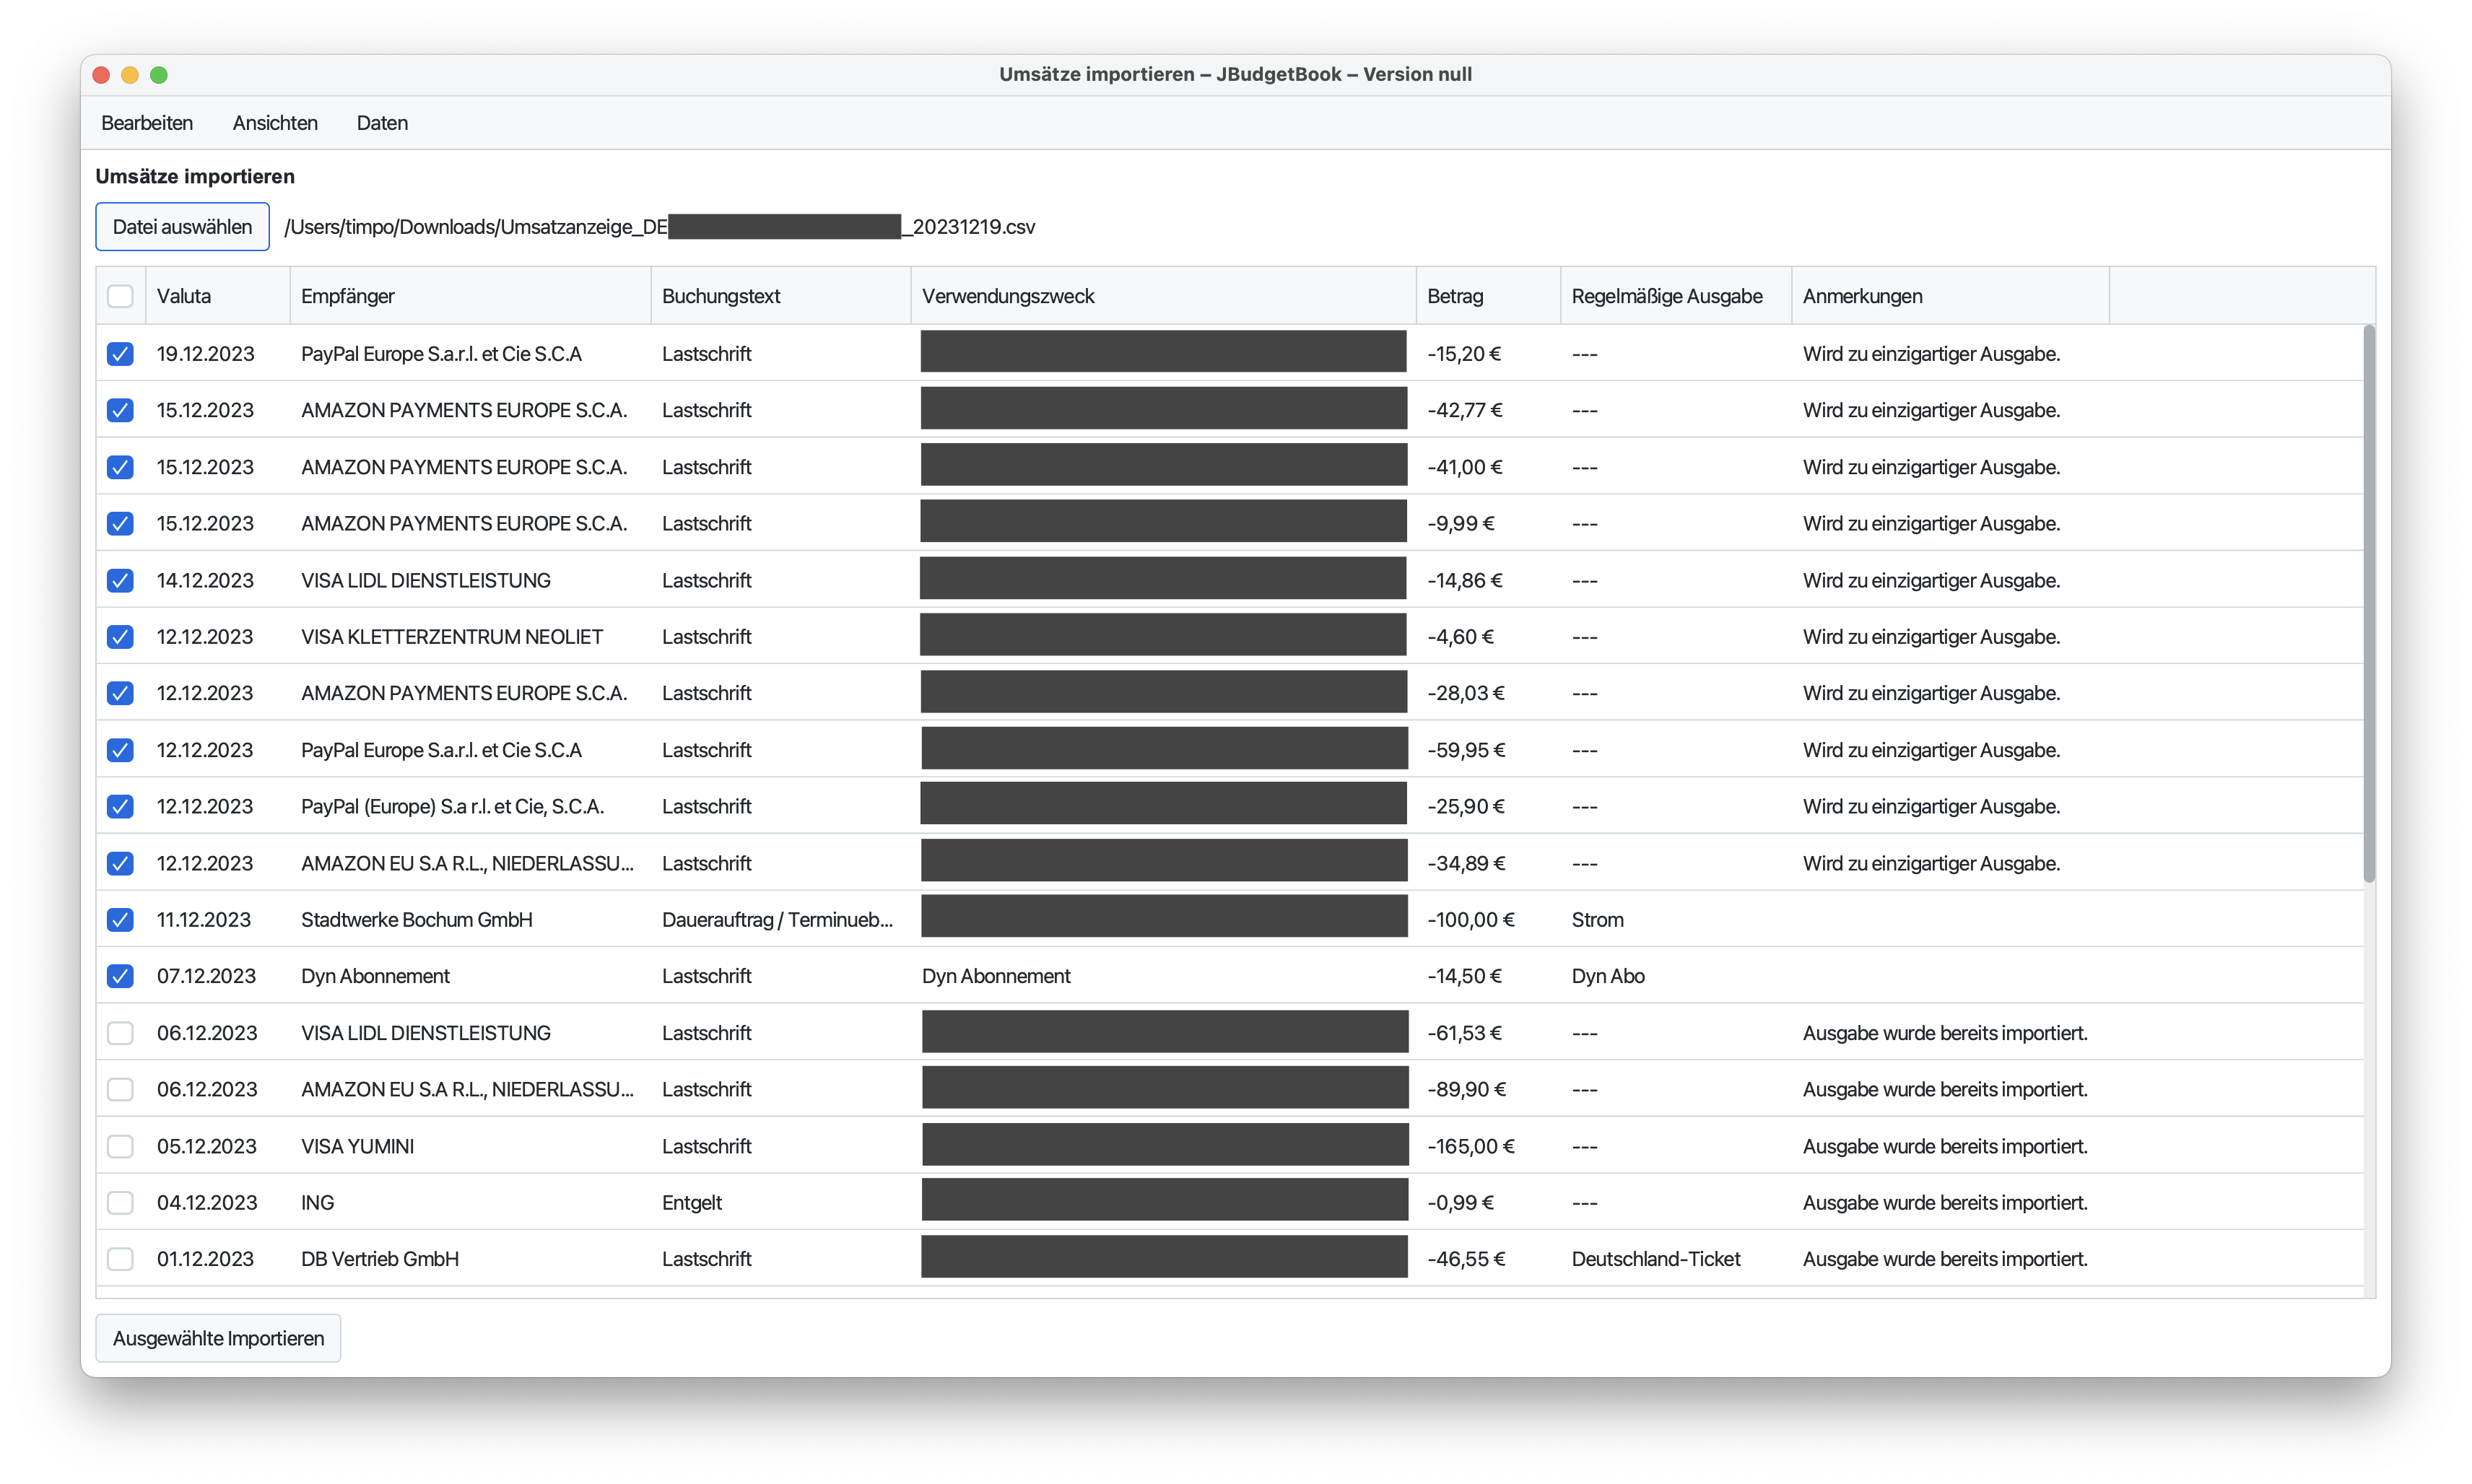
\includegraphics[width=\textwidth]{img/Screenshot-ImportView}
	\vspace{-2em}
	\caption{Ansicht "`Umsätze importieren"'}
	\label{fig:ImportView}
\end{figure}

\section{Importregeln}

Wie reale Umsätze den wiederkehrenden Umsätzen zugeordnet werden sollen, kann in der Detailansicht der wiederkehrenden Umsätze bestimmt werden (s. Abschnitt \ref{sec:fixedExpenses}). Dort kann festgelegt werden, welchen Text der Empfänger oder der Verwendungszweck enthalten muss. Sind Texte in beiden Bedingungen eingetragen, so müssen beide zutreffen (Und-Verknüpfung). 

Sind mehrere Importregeln je wiederkehrendem Umsatz konfiguriert, reicht eine Übereinstimmung aus, damit ein realer Umsatz diesem wiederkehrenden Umsatz zugeordnet wird. 